\section{Introducción}
\subsection{Sistemas de Telecomunicación}
\begin{itemize}
\item\textbf{Telecomunicación:} Comunicación (intercambio de información) a distancia.
\item\textbf{Sistema:} Conjunto de medios y de métodos para el logro de un fin común.
\item\textbf{Red:} Conjunto organizado de recursos tanto físicos como lógicos que permiten la telecomunicación. La red es un recurso escaso que debe compartirse. Para esto se aplican técnicas de acceso múltiple y de multiplexación en las redes.
\item\textbf{Servicio:} Conjunto de medios físicos y lógicos operados y gestionados por un proveedor del servicio, que se ponen a disposición de un cliente, junto con unas normas de acceso y utilización, para satisfacer sus necesidades en materia de Telecomunicaciones.
\end{itemize}
\subsubsection{Clasificación de Servicios}
Los servicios se pueden clasificar atendiendo a los siguientes criterios:
\begin{itemize}
\item Básicos y suplementarios: Los servicios básicos son los que existen por sí mismos, como por ejemplo el servicio telefónico básico, en cambio los suplementarios existen asociados a algún servicio básico, como por ejemplo la identificación de llamada.
\item Clasificación ITU-CCITT: Los servicios portadores son los que transportan la información. Los serviciosfinales o teleservicios incluyen ya el terminal final para poder ofrecer una comunicación completa o añaden capacidades suplementarias como de almacenamiento.
\item Colectivo de usuarios:intercomunicación, comunicación social; comercial, residencial.
\item Capacidad: Banda ancha o estrecha.
\item Modo de efectuar la comunicación: consulta, difusión,conversación, mensajería; simétricos, asimétricos.
\item Movilidad del usuario: movil, portátil, fijo.
\item Tipo de red: RTPC, RDSI, Radiodifusión.
\end{itemize}
\subsubsection{Principales servicios}
\begin{itemize}
	\item Servicio Telefónico: Servicio de comunicación por voz entre usuarios. Es un servicio de gran extensión en el cual se han introducido gran cantidad de avances como la digitalización o la movilidad.
	\item Servicio de transmisión de datos: Servicio de intercambio de información de naturaleza digital que se apoya o en la red telefónica o en la red de datos.
	\item Servicios de valor añadido: Servicios como el fax, el teletexto o el datáfono.
	\item Servicios de radiocomunicación: Servicios caracterizados por la inexistencia de un medio físico de enlace, lo que le permite ser movil y dar acceso a grandes públicos.
\end{itemize}
\subsubsection{Arquitectura de un sistema de Telecomunicación}
En la figura a continuación se pueden ver diferentes entidades funcionales y puntos de referencia (interfaces), interconexiones entre entidades funcionales. Las entidades funcionales son el conjunto de funciones en la red con una finalidad común que pueden comprender uno o varios dispositivos físicos, como los terminales, la red de transporte o la terminación de red. Los puntos de referencia (interfaces) son interconexiones entre entidades, en la figura se ven las interfaces U y S.
\begin{figure}[H]
\centering
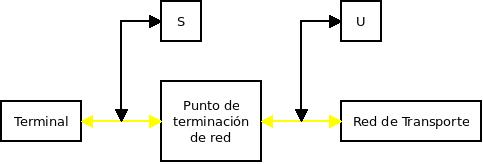
\includegraphics[width=\textwidth]{Imagen/arquisistemateleco.jpg}
\caption{Arquitectura básica de un sistema de Telecomunicación}
\label{}
\end{figure}
\subsection{Organismos reguladores de las Telecomunicaciones}
